\documentclass[12pt,letterpaper]{article}
\usepackage{fullpage}
\usepackage[top=2cm, bottom=4.5cm, left=2.5cm, right=2.5cm]{geometry}
\usepackage{amsmath,amsthm,amsfonts,amssymb,amscd}
\usepackage{lastpage}
\usepackage{enumerate}
\usepackage{fancyhdr}
\usepackage{mathrsfs}
\usepackage{xcolor}
\usepackage{graphicx}
\usepackage{listings}
\usepackage{hyperref}
\usepackage{multicol}

\usepackage{enumitem}


\hypersetup{%
  colorlinks=true,
  linkcolor=blue,
  urlcolor=cyan,
  linkbordercolor={0 0 1}
}
 
\renewcommand\lstlistingname{Algorithm}
\renewcommand\lstlistlistingname{Algorithms}
\def\lstlistingautorefname{Alg.}

\lstdefinestyle{Python}{
    language        = Python,
    frame           = lines, 
    basicstyle      = \footnotesize,
    keywordstyle    = \color{blue},
    stringstyle     = \color{green},
    commentstyle    = \color{red}\ttfamily
}

\setlength{\parindent}{0.0in}
\setlength{\parskip}{0.05in}

% Edit these as appropriate
\newcommand\course{PHYS 243}
\newcommand\hwnumber{4}                  % <-- homework number
\newcommand\MyName{TA: Abtin Shahidi}           % <-- My name

\pagestyle{fancyplain}
\headheight 35pt
\lhead{\MyName}

\chead{\textbf{\Large Homework \hwnumber}}
\rhead{\course \\ Deadline:  20 July 2019, 11:59 pm}
\lfoot{}
\cfoot{}
\rfoot{\small\thepage}
\headsep 1.5em

\begin{document}
\section*{Classify the Handwritten digits!}
In the \href{https://abtinshahidi.github.io/teaching/2019-spring-foundation-machine-learning/week7}{week7} course, we used one of the most interesting data sets and that is the MNIST handwritten data set. You can find the data set following the notebook or you can directly get it from \href{http://yann.lecun.com/exdb/mnist/}{here}. Also, you do not have to use the whole dataset if there is a computation limit.

The task here is to classify the digits into their own category.

\subsection*{Find all the 9s!}
In this section you should build up a classifier that can distinguish number 9 from every other numbers. (reusing code and libraries are ok as long as you explain what is going on)

For each section below you need to measure your performance. So, make sure to run the performance check at every part.

\begin{enumerate}
\item Find the 9s using K-Nearest neighbours for Minkowski metric of order (1, 2, 3). 
\item Find the 9s using Decision tree. 
\item Find the 9s using Random Forests.
\end{enumerate}

\begin{figure}[ht]
\begin{center}
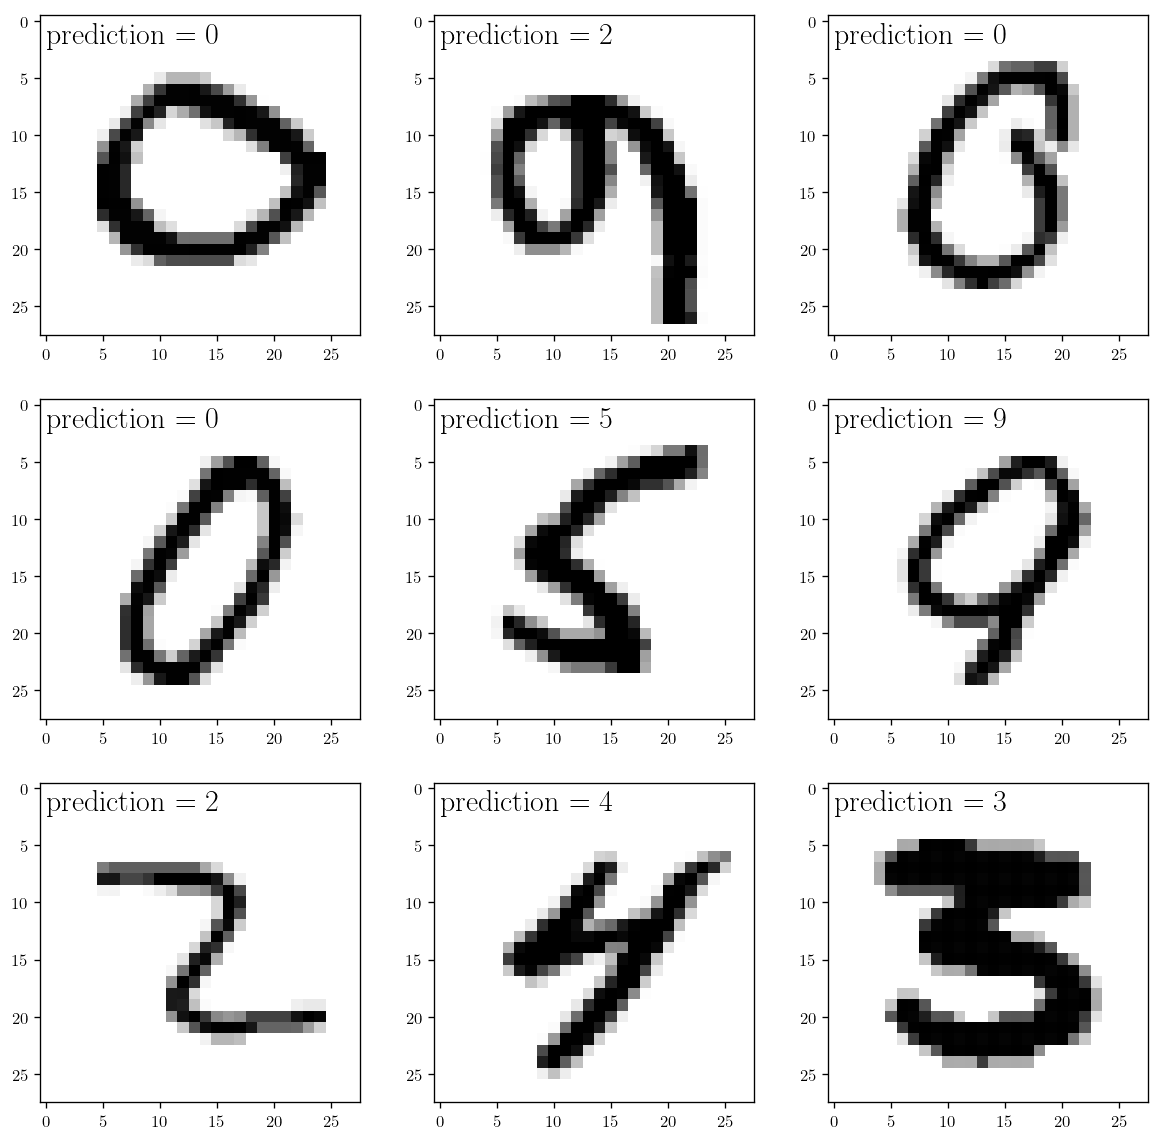
\includegraphics[scale=0.35]{week7_98_0.png}
\end{center}
\caption{Our SVM implementation prediction vs the digit}
\end{figure}

\subsection*{Find every single digits!}
\begin{enumerate}
\item First forget about the labels and run the k-means algorithm to find whether there is an underlying patterns. So, first find the $k$ clusters (here is obviously $10$ clusters). Then look at their labels and find the accuracy. By doing this you are turning a supervised learning into an unsupervised learning! 

\item Find the digits using K-Nearest neighbours for Minkowski metric of order (1, 2, 3). 
\item Find the digits using Decision tree. 
\item Find the digits using Random Forests.

\item Comment on any significant difference between your results for the \textbf{binary classifier} vs \textbf{multi-class classifier}s.
\end{enumerate}




\end{document}


